\section{Evklidske in origami konstrukcije}

Kraj in čas izvora origamija nista jasno določena. Nekateri viri zatrjujejo, da izhaja iz Japonske, drugi ga pripisujejo Kitajski, tretji se ne strinjajo z nobeno od teh dveh možnosti. Verjetno so umetnost zlaganja odkrili še pred izumom papirja, za katerega je l. 105 po Kr. poskrbel kitajski dvorni uradnik Cai Lun, saj se da npr.\ zlagati tudi robce iz blaga~\cite{robinson2024}. Je pa papir idealen material za zlaganje. Japonska beseda \emph{origami} kot umetnost zgibanja papirja (``oru'' -- prepogibati, ``kami'' -- papir) se je na Daljnem vzhodu začela uporabljati proti koncu 19. stoletja.

Povečano zanimanje za origami v matematiki se je začelo v 2.\ pol.\ 20.\ stoletja in s seboj prineslo množično izhajanje literature o povezavi origamija z matematiko, fiziko, astronomijo, računalništvom, kemijo in še mnogimi drugimi vedami~\cite{zore2022}. V angleščini je tako za matematično raziskovanje s prepogibanjem papirja nastalo poimenovanje ``\emph{origamics}''. V slovenščini uradnega prevoda še ni, Grahor pa v~\cite[str.\ 5]{sgv2016} po zgledu poimenovanj veliko znanstvenih disciplin (\emph{mathematics} -- matematika, \emph{physics} -- fizika itd.) predlaga termin ``origamika''.

\subsection{Evklidovi postulati in evklidske konstrukcije}

Preden si pogledamo, kaj lahko s prepogibanjem papirja konstruiramo, se spomnimo, na čem temelji evklidska geometrija. Za njenega očeta štejemo grškega matematika Evklida\footnote{O življenju tega aleksandrijskega učenjaka ne vemo nič gotovega, je pa zelo verjetno živel za časa prvega Ptolemaja (faraon v času 306--283 pr.\ Kr.)~\cite[str.\ 61]{struik1986}.}, ki je napisal zelo znano zbirko trinajstih knjig pod skupnim imenom \emph{Elementi}. V njih obravnavana snov temelji na strogo logični izpeljavi izrekov iz definicij\footnote{\emph{Definicija} je nedvoumno jasna opredelitev novega pojma.}, aksiomov\footnote{\emph{Aksiom} je temeljna resnica ali načelo, ki ne potrebuje dokazov (oz.\ dokaz sploh ne obstaja) in vedno velja.} in postulatov\footnote{\emph{Postulat} je predpostavka oz.\ zahteva. Evklid med aksiomi in postulati ni postavil jasne razlike, Aristotel pa je postulat od aksioma ločil po tem, da gre pri prvem bolj za hipotezo kot temeljno resnico, vendar se njene veljavnosti ne dokazuje, temveč privzame kot veljavno~\cite[str.\ 122]{euclidI}. V primeru petega Evklidovega postulata se bomo spomnili, da nam to, ali ga privzamemo ali ne, poda različne geometrije. Danes med pojmoma ne ločujemo~\cite[str.\ 2]{geometricconstructions}.}. Še danes večina osnovno- in srednješolske geometrije izvira prav iz prvih šestih knjig Elementov.

Prva knjiga nas še posebej zanima. V njej je Evklid najprej definiral osnovne pojme -- točka, premica, površina, ravnina, ravninski kot, pravi kot, ostri kot, topi kot, krog, središče kroga, premer, enakostranični in enakokraki trikotnik, kvadrat \ldots ter nazadnje upeljal še pojem vzporednih premic~\cite{euclidI}. Nato je zapisal znamenitih pet postulatov, iz katerih izhaja vsa evklidska geometrija:

\renewcommand{\thepostulat}{P\arabic{postulat}}

\begin{postulat}
    \label{post:P1}
    Med dvema poljubnima točkama je mogoče narisati ravno črto.
\end{postulat}
\begin{postulat}
    \label{post:P2}
    Vsako ravno črto je mogoče na obeh koncih podaljšati.
\end{postulat}
\begin{postulat}
    \label{post:P3}
    Mogoče je narisati krožnico s poljubnim središčem in poljubnim polmerom.
\end{postulat}
\begin{postulat}
    \label{post:P4}
    Vsi pravi koti so med seboj skladni.
\end{postulat}
\begin{postulat}
    \label{post:P5}
    Če poljubni ravni črti sekamo s tretjo ravno črto (prečnico) in je vsota notranjih kotov eni strani prečnice manjša od dveh pravih kotov, potem se dani premici, če ju dovolj podaljšamo, sekata na tej strani prečnice.
    \opomba{Vemo že, da je postulat~\ref{post:P5} ekvivalenten \emph{aksiomu o vzporednicah}, ki pravi, da skozi dano točko, ki ne leži na dani premici, poteka natanko ena vzporednica k tej premici.}
\end{postulat}

\begin{definicija}
    \emph{Evklidske konstrukcije} so konstrukcije premic, kotov, krožnic in drugih geometrijskih figur, ki jih je mogoče konstruirati le z uporabo t.\ i.\ \emph{evklidskih orodij}:
    \begin{itemize}
        \item neoznačeno in neskončno dolgo ravnilo (angl.\ \emph{straightedge})
        \item šestilo, ki ne prenaša razdalj (ko ga dvignemo od podlage, se njegova kraka zložita skupaj)
    \end{itemize}
\end{definicija}

\begin{opomba}
    Da se pokazati, da lahko za konstrukcije ekvivalentno uporabimo tudi šestilo, ki prenaša razdalje~\cite[str.\ 6--7]{geometricconstructions}. Zato imamo odslej z izrazom \emph{šestilo} v mislih kar moderno šolsko šestilo.
\end{opomba}

Formalno so torej edine dovoljene operacije tiste iz postulatov~\ref{post:P1}--\ref{post:P3}. Seveda privzamemo, da so konstruktibilne tudi točke, ki jih dobimo kot že dane ali kot presečišča dveh premic, dveh krožnic ali premice in krožnice. Vendar je to dovolj, da lahko le z neoznačenim ravnilom in šestilom konstruiramo premice, kote, simetrale kotov in daljic, krožnice in še mnogo drugega. V resnici se da skonstruirati toliko geometrijskih figur, da se matematiki raje vprašamo, česa pa se s tem orodjem \emph{ne} da skonstruirati. In tu pridemo do motivacije za uvedbo origami konstrukcij, saj lahko z njimi npr.\ rešimo kar dva od treh znamenitih starogrških problemov, ki jih z evklidskim orodjem ne moremo (gl.\ poglavje~\ref{pogl:starogrskiproblemi}).

\subsection{Origami konstrukcije}
\label{origami_konstrukcije}

V nalogi se bomo omejili le na prepogibanje v ravnini. Za model evklidske ravnine vzamemo kvadraten list papirja, saj s prepogibanjem očitno v tej ravnini tudi ostanemo. Dogovorimo se, da pregibe konsktruiramo le po enega naenkrat ter v ravni črti, po vsakem prepogibu papir znova odgrnemo in prepovedana je uporaba kakršnegakoli orodja (npr.\ škarje in lepilo).  Bralec je ob branju povabljen, da opisane konstrukcije tudi sam preizkusi na listu papirja, sicer pa se jih da brez večjih težav predstavljati tudi brez fizičnega materiala. Pri izbiri papirja je priporočljiv rahlo prosojen papir, skozi katerega se vidijo morebitne označbe točk in premic s svinčnikom (npr.\ navaden kuhinjski papir za peko).

Ker so pregibi torej ravne črte, nam služijo kot modeli premic. Na začetku, ko imamo pred seboj le kvadraten list papirja, so naše premice njegove stranice. Nove premice so pregibi skozi točke. Začetni modeli točk so ravno oglišča našega lista papirja, nadaljne točke pa dobimo kot presečišča premic, torej presečišča pregibov, ki gredo skozi dane ali že skonstruirane točke. Torej imamo le pet možnosti, kako prepogniti papir -- tako, da zložimo (slikovni prikaz v~\cite[str.\ 25--26]{hull2020}):
\begin{itemize}
    \item točko na drugo točko (en možen pregib),
    \item točko samo vase (neskončno možnih pregibov),
    \item točko na premico (neskončno možnih pregibov),
    \item premico na drugo premico (en ali dva možna pregiba) in
    \item premico samo vase (neskončno možnih pregibov).
\end{itemize}

\begin{definicija}
    Vzemimo kvadraten list papirja. Začetne premice so njegove stranice, začetne točke pa njegova oglišča. Nove premice so pregibi papirja skozi dane ali že skonstruirane točke, nove točke pa so presečišča premic oz.\ pregibov. Konstrukcije, ki jih izvajamo z z zgoraj naštetimi ter ravnimi in enkratnimi pregibi, imenujemo \emph{origami konstrukcije}.
\end{definicija}

\subsubsection{Origami operacije}
\label{podpodpogl:operacije}

V zadnjem stoletju se je preko različnih matematikov (Jacques Justin, Peter Messer, Benedetto Scimemi, Humiaki Huzita, Koshiro Hatori, George E.\ Martin idr.; nekateri so med seboj sodelovali, drugi so delovali neodvisno) izoblikoval seznam operacij, ki nam jih omogočajo zgoraj naštete konstrukcije. Seznam se je med avtorji razlikoval v številu (gl.\ ~\cite[str.\ 29--30]{hull2020}), skupno pa se je izoblikovalo osem -- na prvi pogled različnih -- operacij. Najprej jih naštejmo, potem pa si ob sledečih slikah poglejmo še prikaz opisanih konstrukcij. Videli bomo, da moramo pri nekaterih operacijah ločiti več primerov~\cite{michael2005, zore2022}.

\renewcommand{\theoperacija}{O\arabic{operacija}}

\begin{operacija}
    \label{op:O1}
    Za poljubni točki $A$ in $B$ obstaja natanko en pregib $p$, ki gre skoznju.
\end{operacija}
\begin{operacija}
    \label{op:O2}
    Za poljubni premici lahko določimo njuno presečišče, če obstaja.
\end{operacija}
\begin{operacija}
    \label{op:O3}
    Za poljubni točki $A$ in $B$ obstaja natanko en pregib $p$, da se točki pokrijeta.
\end{operacija}
\begin{operacija}
    \label{op:O4}
    Za poljubni premici $a$ in $b$ obstaja pregib $p$, ki ju položi eno na drugo.
\end{operacija}
\begin{operacija}
    \label{op:O5}
    Za poljubno točko $A$ in premico $a$ obstaja natanko en pregib $p$ skozi točko $A$, ki je pravokoten na premico $a$.
\end{operacija}
\begin{operacija}
    \label{op:O6}
    Za primerno izbrani točki $A$ in $B$ ter premico $a$ obstaja pregib $p$ skozi točko $B$, ki točko $A$ položi na premico $a$.
\end{operacija}
\begin{operacija}
    \label{op:O7}
    Za primerno izbrani točki $A$ in $B$ ter premici $a$ in $b$ obstaja pregib $p$, ki točko $A$ položi na premico $a$ in točko $B$ na premico $b$.
\end{operacija}
\begin{operacija}
    \label{op:O8}
    Za poljubno točko $A$ ter nevzporedni premici $a$ in $b$ obstaja pregib $p$, ki je pravokoten na premico $b$ in točko $A$ položi na premico $a$.
\end{operacija}

Sedaj za vsako operacijo posebej poglejmo njeno konstrukcijo. Takoj opazimo, da je operacija~\ref{op:O1} ekvivalentna postulatu~\ref{post:P1}, kar nam lahko vzbudi zanimanje za povezavo med evklidskimi in origami konstrukcijami. Operacija~\ref{op:O2} je izvedljiva v vsakem primeru nevzporednih pregibov in nam omogoča določitev novih točk v našem modelu ravnine. Operacija~\ref{op:O3} pa nam poda konstrukcijo simetrale daljice $AB$ (slika~\ref{fig:O1-O3}) -- ko opravimo pregib in pustimo papir še zapognjen, je očitno, da so točke na pregibu enako oddaljene od točk $A$ in $B$.

\begin{figure}[h]
    \centering
    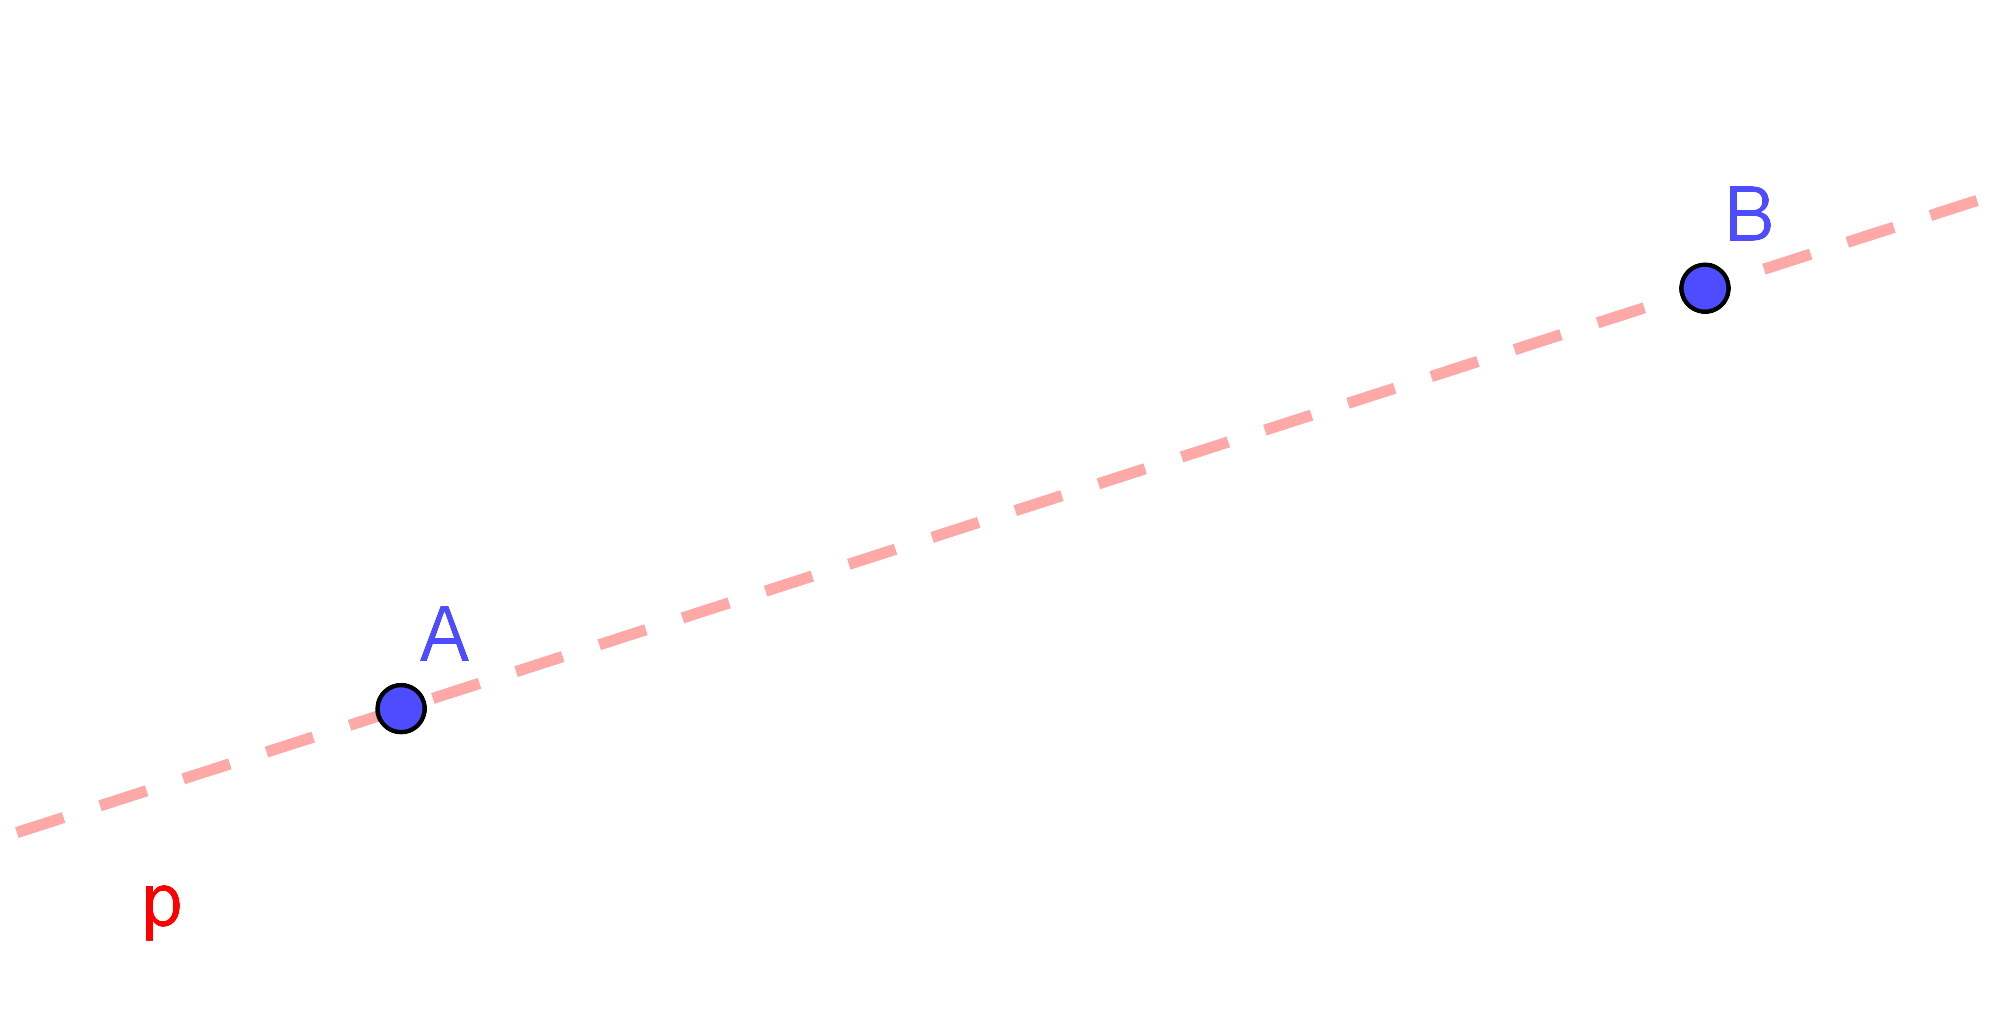
\includegraphics[width=0.4\textwidth]{images/origami_operacije/O1.png}
    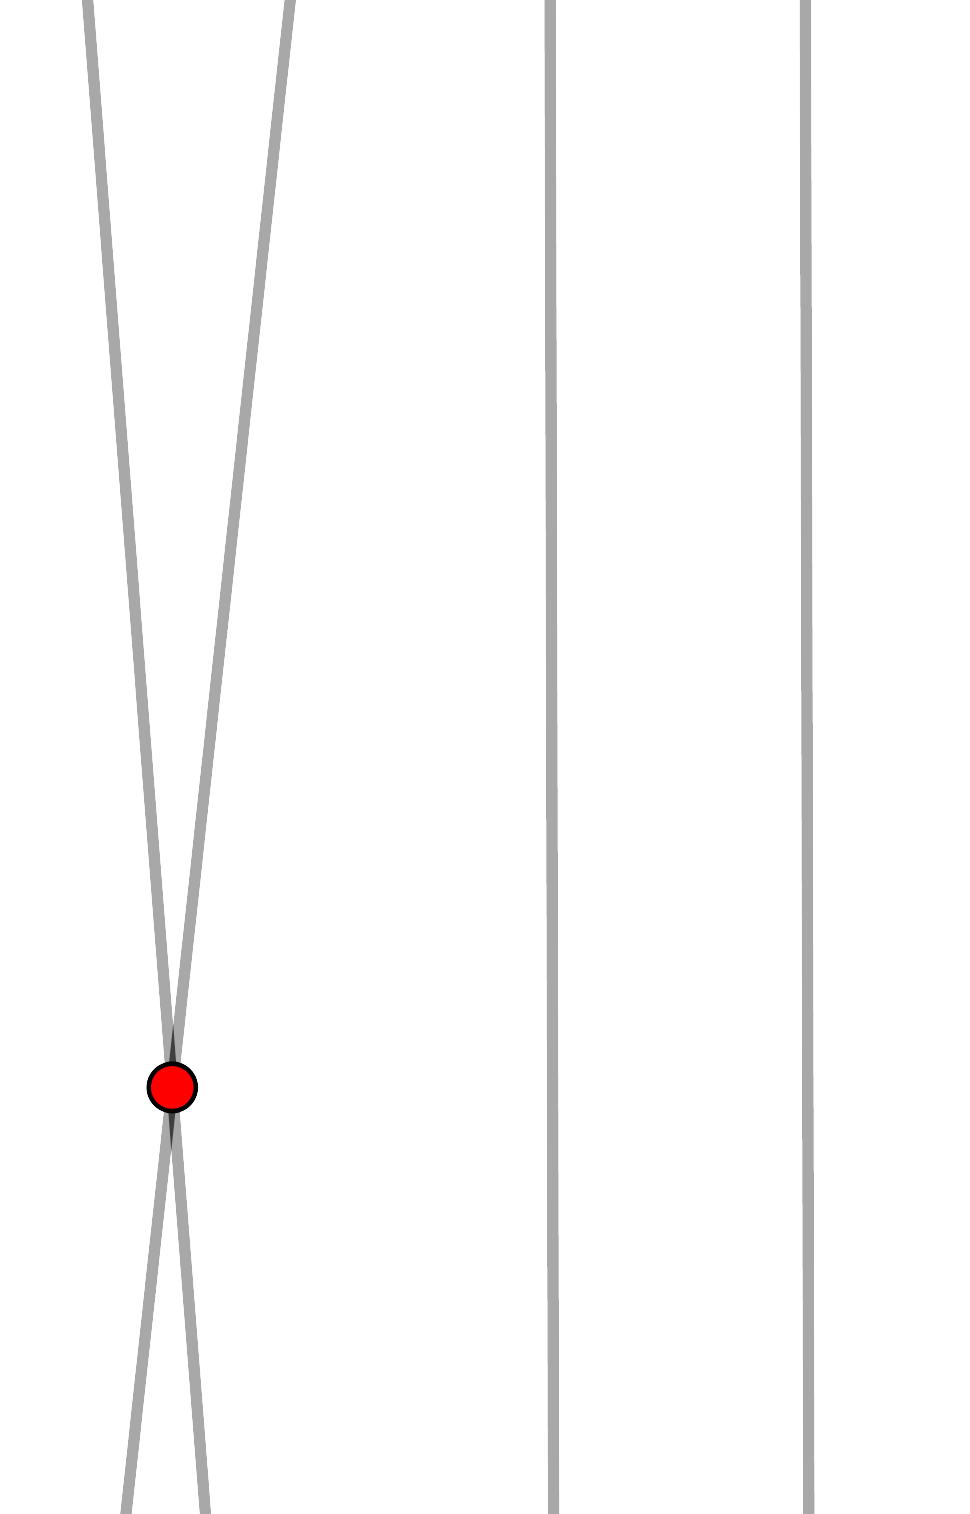
\includegraphics[width=0.2\textwidth]{images/origami_operacije/O2.png}
    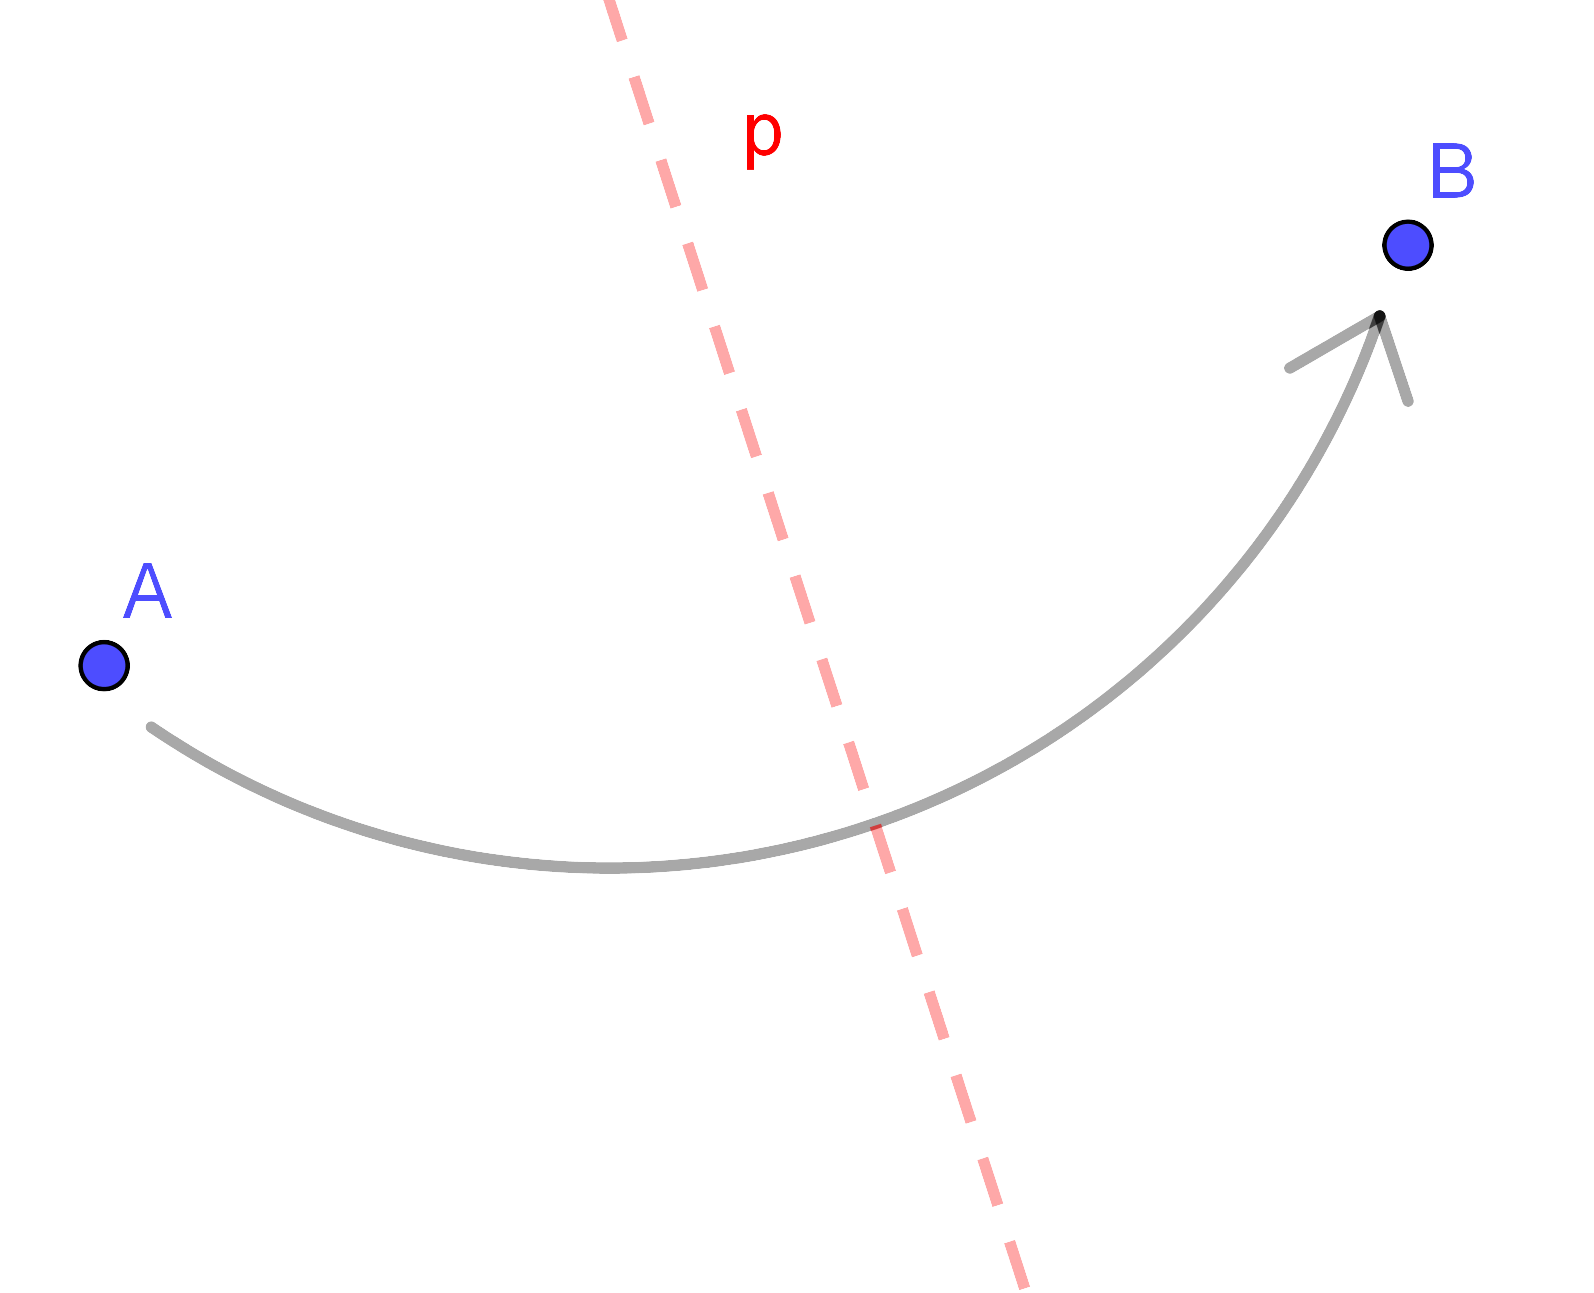
\includegraphics[width=0.35\textwidth]{images/origami_operacije/O3.png}
    \caption[Operacije~\ref{op:O1},~\ref{op:O2} in~\ref{op:O3}]{Operacije (od leve proti desni)~\ref{op:O1},~\ref{op:O2} in~\ref{op:O3}.}
    \label{fig:O1-O3}
\end{figure}

Nadalje opazimo, da nam operacija~\ref{op:O4} konstruira obe simetrali kota, ki ga določata premici in njuno presečišče, v primeru vzporednih premic pa dobimo tretjo vzporednico, ki leži na sredi med njima (slika~\ref{fig:O4}). Zato sta tu možna po dva ali, v posebnem primeru, en pregib.

\begin{figure}[h]
    \centering
    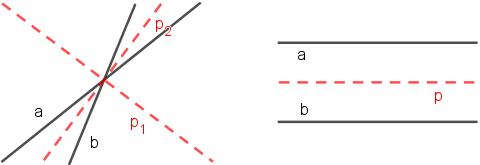
\includegraphics[width=0.5\textwidth]{images/origami_operacije/O4.png}
    \caption[Operacija~\ref{op:O4}]{Operacija~\ref{op:O4} v obeh možnih primerih.}
    \label{fig:O4}
\end{figure}

Operacija~\ref{op:O5} nam podaja konstrukcijo pravokotnice na premico skozi dano točko (slika~\ref{fig:O5}). Pri tem je vseeno, ali točka leži na premici ali ne. Pregib opravimo tako, da premico položimo samo nase in pazimo, da je točka $A$ v pregibu. Zaradi simetrije je pregib res pravokoten na premico in tako tudi en sam.

\begin{figure}[h]
    \centering
    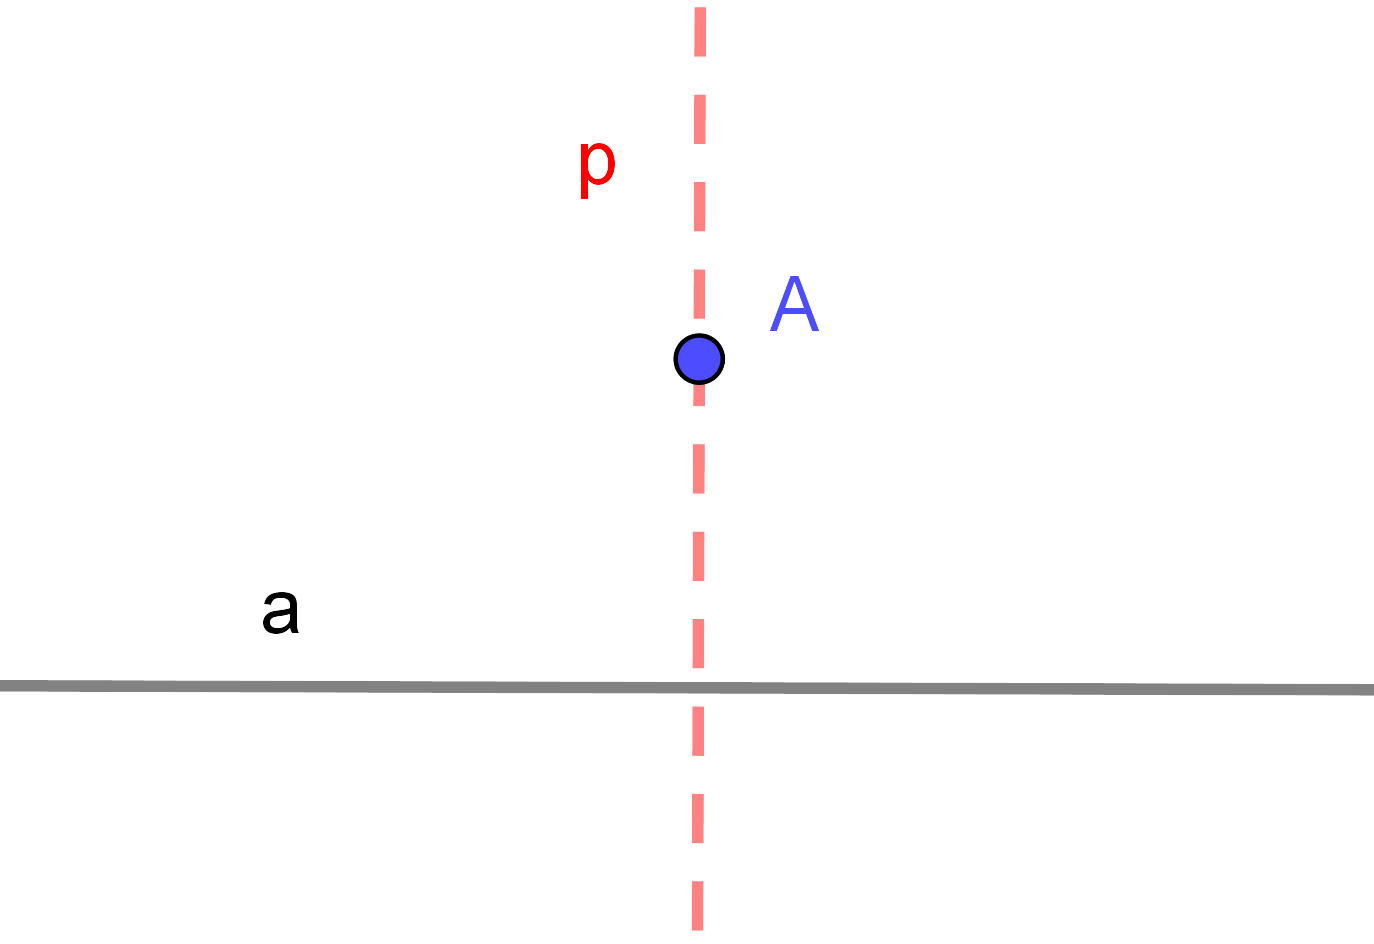
\includegraphics[width=0.35\textwidth]{images/origami_operacije/O5.png}
    \caption[Operacija~\ref{op:O5}]{Operacija~\ref{op:O5}.}
    \label{fig:O5}
\end{figure}

Operacija~\ref{op:O6} je še posebej zanimiva. Najprej si poglejmo njeno konstrukcijo. Vzemimo točki $A$ in $B$ ter premico $a$. Iščemo pregib skozi $B$, ki $A$ položi na premico $a$. Ker točka $B$ leži na pregibu, je enako oddaljena tako od točke $A$ kot tudi njene slike $A'$ na premici $a$, torej je $A'$ ravno presečišče premice $a$ in krožnice s središčem v $B$ ter polmerom $AB$. Pregib je simetrala daljice $AA'$, ki po konstrukciji poteka skozi točko $B$. Če velja $ d(A,B) > d(B,a) $, sta presečišči s premico $a$ dve (in s tem tudi dva možna pregiba, gl.\ sliko~\ref{fig:O6} levo), v primeru $ d(A,B) = d(B,a) $ je presečišče eno samo (in s tem en možen pregib, gl.\ sliko~\ref{fig:O6} na sredi) in je premica $a$ takrat tangentna na omenjeno krožnico, v zadnjem primeru, ko velja $ d(A,B) < d(B,a) $, pa presečišč ni (in s tem tudi pregiba, gl.\ sliko~\ref{fig:O6} desno).

\begin{figure}[h]
    \centering
    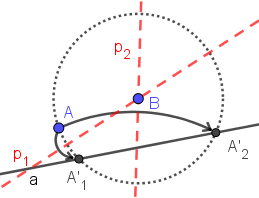
\includegraphics[width=0.55\textwidth]{images/origami_operacije/O6a.png}
    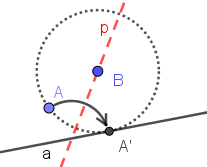
\includegraphics[width=0.2\textwidth]{images/origami_operacije/O6b.png}
    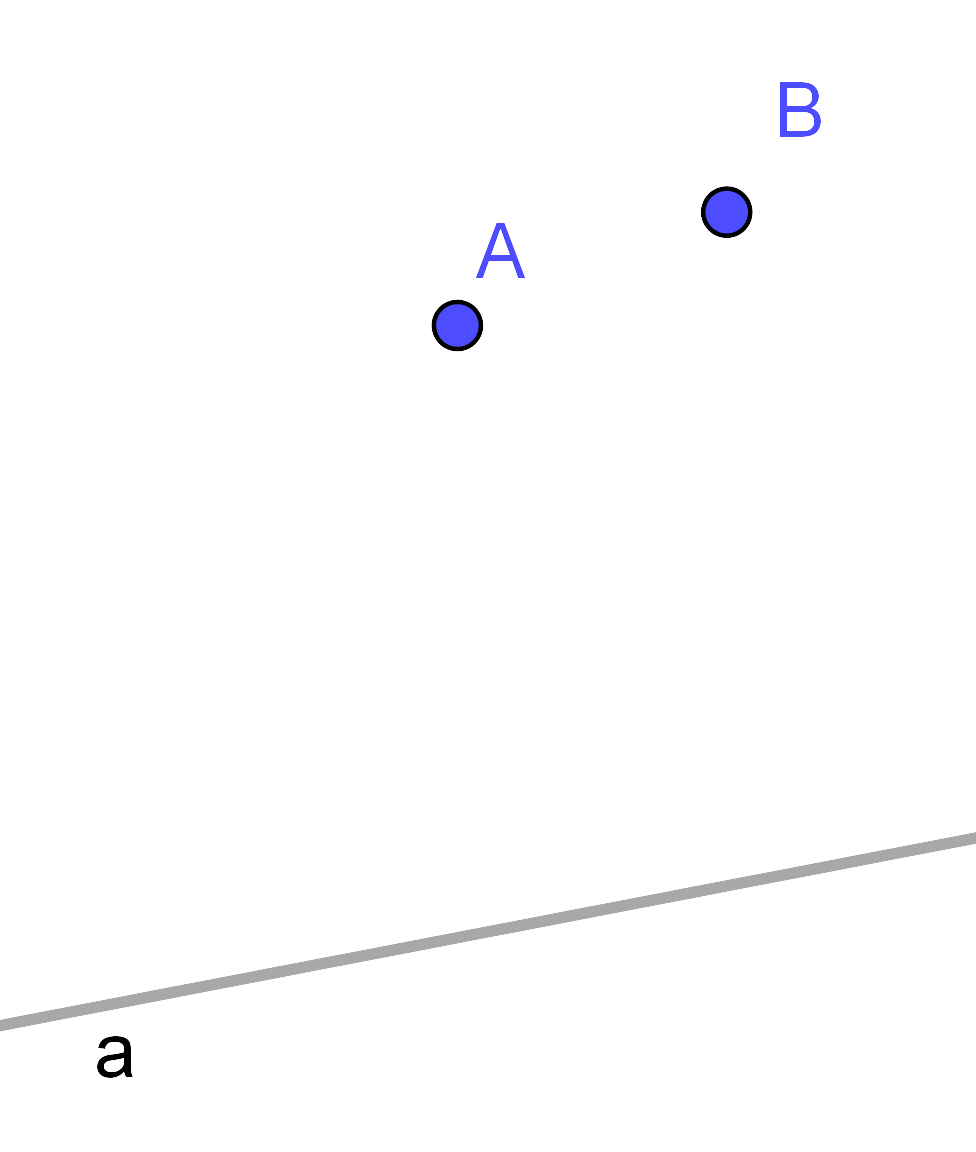
\includegraphics[width=0.2\textwidth]{images/origami_operacije/O6c.png}
    \caption[Operacija~\ref{op:O6}]{Operacija~\ref{op:O6} v vseh treh primerih.}
    \label{fig:O6}
\end{figure}

Zgodba operacije~\ref{op:O6} se tu še ne zaključi. Ker na pregibu ležijo vse točke, ki so enako oddaljene od točke $A$ in $A'$, to velja tudi za točko $P$, ki jo dobimo kot presečišče pregiba in pravokotnice na premico $a$ skozi $A'$. Zanjo velja $ d(A,P) = d(P,a) $ in je enolično določena (v srednjem primeru na sliki~\ref{fig:O6} je to kar točka $B$). Torej točka $P$ leži na paraboli z goriščem $A$ in premico vodnico $a$. Ker pregib seka parabolo le v tej točki ($P$ je edina enako oddaljena od gorišča in vodnice), smo s tem skonstuirali ravno \emph{tangento na to parabolo} (slika~\ref{fig:O6_parabola}). V levem primeru na sliki~\ref{fig:O6_parabola} smo dobili dve tangenti.

\begin{figure}[h]
    \centering
    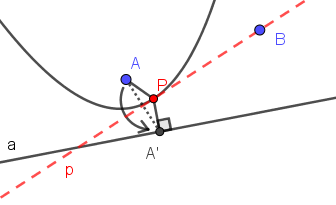
\includegraphics[width=0.6\textwidth]{images/origami_operacije/O6_parabola.png}
    \caption[Tangenta na parabolo]{Operacija~\ref{op:O6} kot konstrukcija tangente na parabolo z goriščem v $A$ in premico vodnico $a$.}
    \label{fig:O6_parabola}
\end{figure}

Poglejmo si naslednjo operacijo. Konstrukcijo~\ref{op:O7} začnemo z upogibom papirja, ki točko $A$ položi na premico $a$, potem pa točko premikamo po premici, dokler se tudi točka $B$ ne stakne s premico $b$. Takrat naredimo pregib. Za enako izbiro točk in premic je lahko možnih več pregibov (gl.\ sliko~\ref{fig:O7}), če pa sta premici vzporedni in je njuna medsebojna razdalja večja od razdalje med točkama, pregib sploh ne obstaja (to lahko bralec ugotovi ob preprostem razmisleku, kako se giba točka $B$ med premikanjem točke $A$ po premici $a$).

\begin{figure}[h]
    \centering
    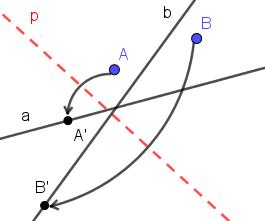
\includegraphics[width=0.35\textwidth]{images/origami_operacije/O7b.png}
    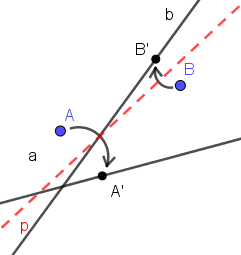
\includegraphics[width=0.3\textwidth]{images/origami_operacije/O7a.png}
    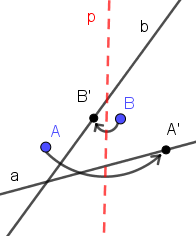
\includegraphics[width=0.3\textwidth]{images/origami_operacije/O7c.png}
    \caption[Operacija~\ref{op:O7}]{Operacija~\ref{op:O7} (primer treh pregibov za isti točki in premici).}
    \label{fig:O7}
\end{figure}

Kaj je geometrijski pomen te operacije? Če smo pri operaciji~\ref{op:O6} dobili tangento na parabolo, potem lahko takoj vidimo, da pri operaciji~\ref{op:O7} dobimo \emph{skupno tangento na dve paraboli} -- ena ima gorišče v točki $A$ in premico vodnico $a$, druga pa gorišče v točki $B$ ter premico vodnico $b$ (slika~\ref{fig:O7_paraboli}).

\begin{figure}[h]
    \centering
    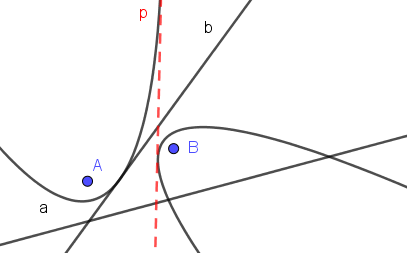
\includegraphics[width=0.7\textwidth]{images/origami_operacije/O7c_paraboli.png}
    \caption[Skupna tangenta na dve paraboli]{Operacija~\ref{op:O7} kot konstrukcija skupne tangente na dve paraboli.}
    \label{fig:O7_paraboli}
\end{figure}

\begin{opomba}
    O operaciji~\ref{op:O7} naj bi prva pisala italijanski matematičarki Margherita P.\ Beloch, po kateri operacijo imenujemo tudi \emph{Belochin pregib}.
\end{opomba}

Zadnja operacija~\ref{op:O8} zahteva nevzporedni premici, saj v nasprotnem primeru ne moremo konstruirati pregiba, ki bi bil pravokoten na obe premici in točko $A$ položil na premico $a$ (razen če le-ta že leži na njej). Premislimo geometrijsko konstrukcijo: ker mora biti pregib pravokoten na premico $b$, bo slika točke $A$ (označena z $A'$) ležala na vzporednici skozi točko $A$ k premici $b$. Prav tako mora točka $A'$ ležati na premici $a$, torej je slika ravno presečišče omenjene vzporednice in premice $a$. Iskan pregib je simetrala daljice $AA'$, ki je po konstrukciji pravokoten na premico $b$ (slika~\ref{fig:O8}).

\begin{figure}[h]
    \centering
    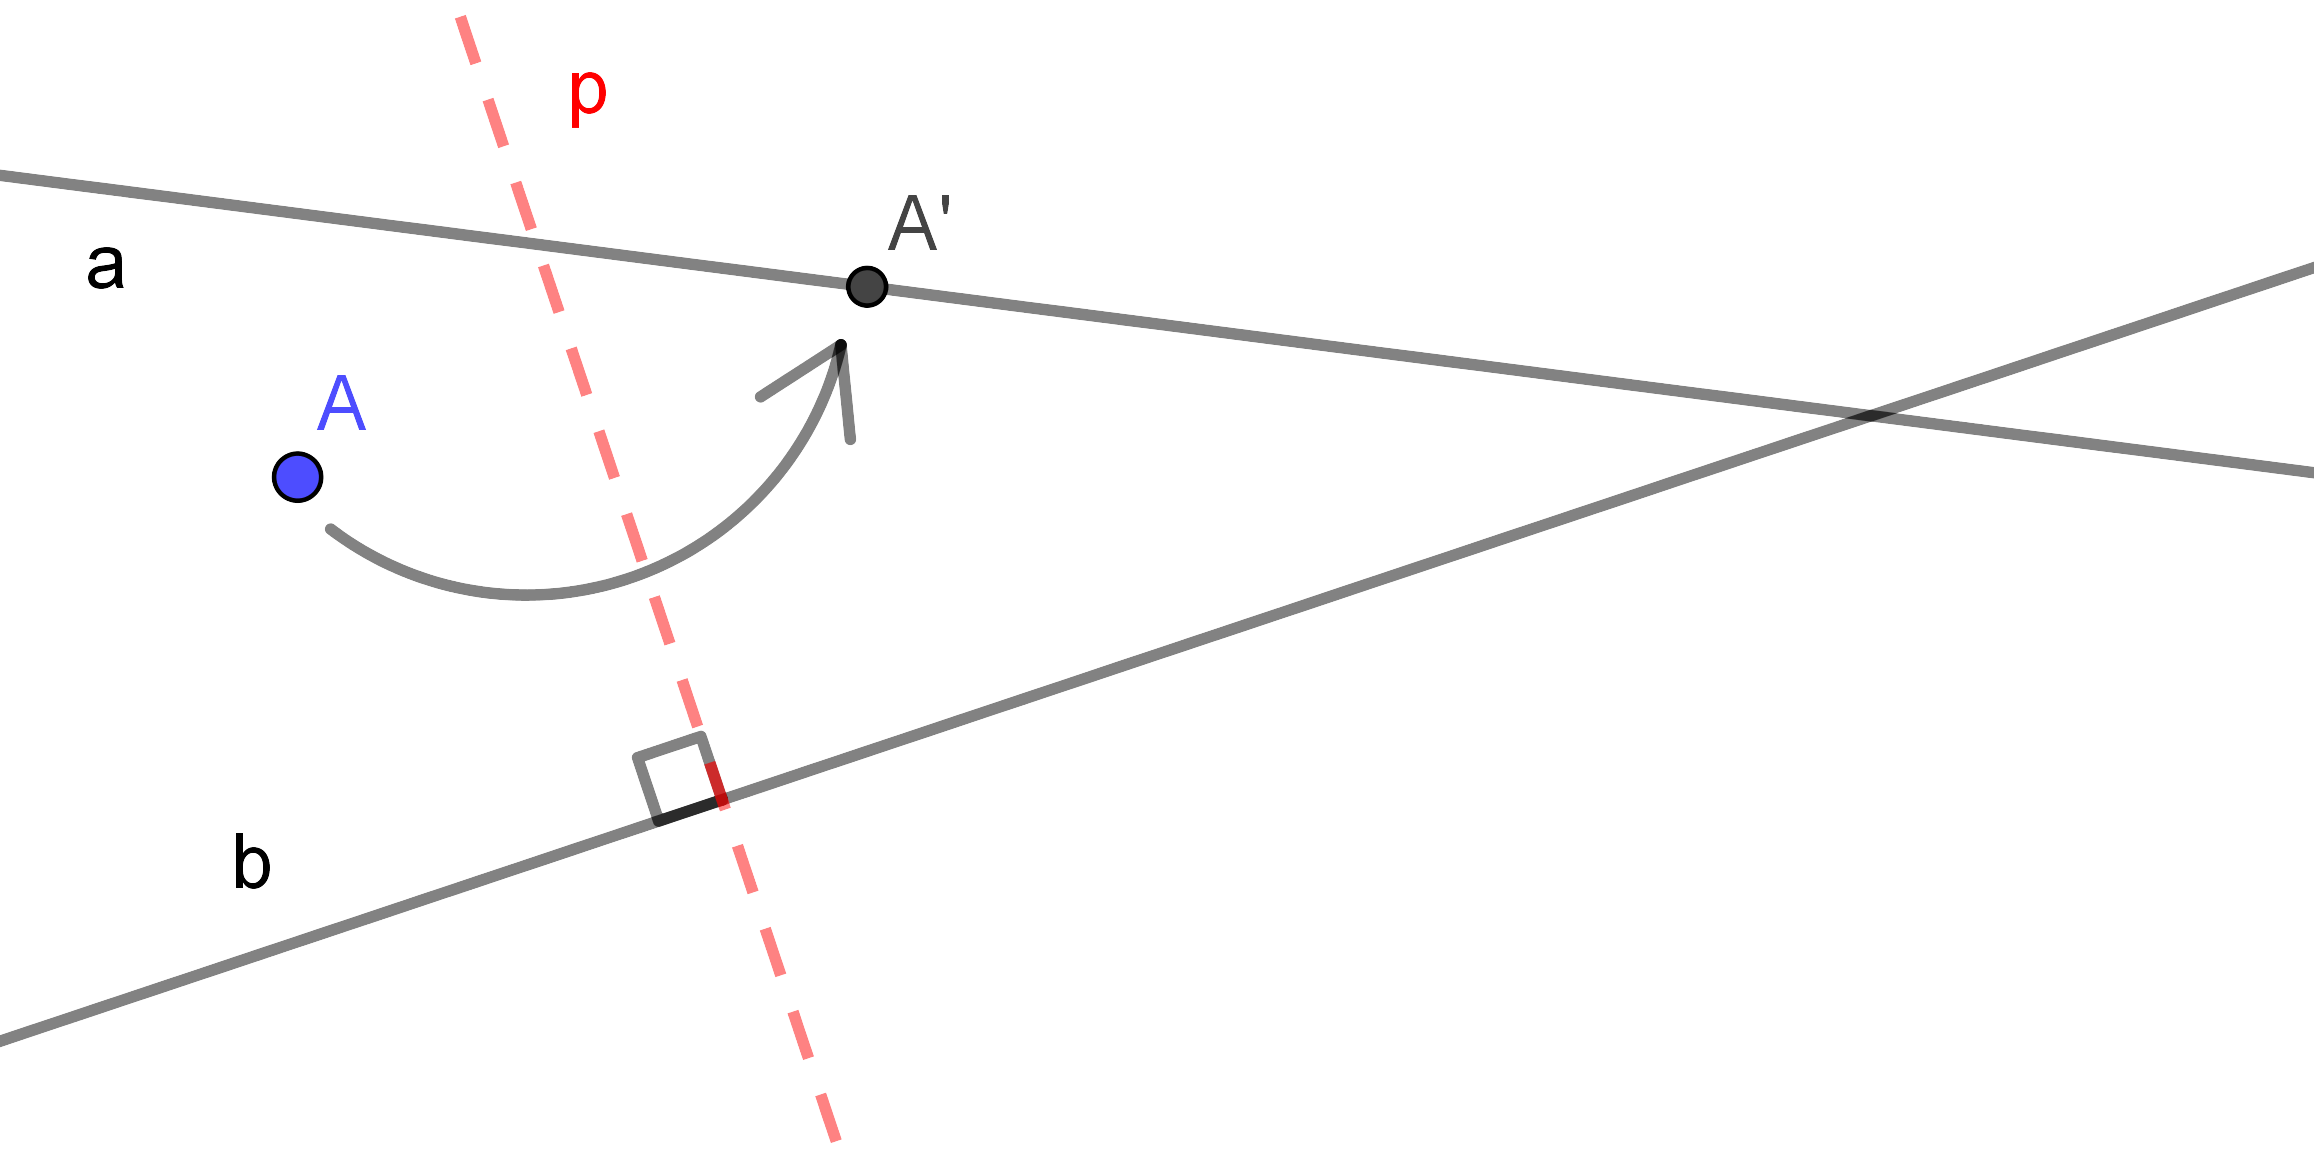
\includegraphics[width=0.6\textwidth]{images/origami_operacije/O8.png}
    \caption[Operacija~\ref{op:O8}]{Operacija~\ref{op:O8}.}
    \label{fig:O8}
\end{figure}

\subsubsection{Zadostne in potrebne origami operacije}

Izkaže se, da je teh osem operacij zadostnih za katerokoli origami konstrukcijo.

\begin{izrek}
    \label{izr:op1do8}
    Če dovolimo le enkratne in ravne pregibe, so edine možne operacije prepogibanja operacije~\ref{op:O1}--\ref{op:O8}.
\end{izrek}

Ideja dokaza je, da za vsak možen prepogib, ki prekrije točko ali premico s točko ali premico (gl.\ seznam na začetku podpoglavja \ref{origami_konstrukcije}) pogledamo vse možnosti. Izkaže se, da res dobimo prepogibe iz operacij~\ref{op:O1}--\ref{op:O8}. Za natančen dokaz s slikovno ponazoritvijo gl.\ \cite[str.\ 24--26 (izrek 1.1)]{hull2020}.

Vendar ali so vse te operacije tudi potrebne ali lahko kakšno izpustimo? Operacija~\ref{op:O2} je očitno potrebna, saj nam določa nove točke. Če podrobneje opazujemo ostale konstrukcije, pa opazimo, da so vse posebni primeri operacije~\ref{op:O7} (t.\ j.\ konstrukcija pregiba, ki točko $A$ položi na premico $a$ in točko $B$ na premico $b$), ko premici $a$ in $b$ sovpadata ali ko ena ali obe izmed točk $A$ in $B$ ležita na premici:
\begin{itemize}
    \item Operacija~\ref{op:O1}: Naj točka $A$ leži na premici $a$, točka $B$ pa na premici $b$. Pregib skozi točki $A$ in $B$ točko $A$ ohrani na premici $a$ in točko $B$ na premici $b$.
    \item Operacija~\ref{op:O3}: Naj točka $A$ leži na premici $b$, točka $B$ pa na premici $a$. Pregib, ki položi točki drugo na drugo, točko $A$ položi na premico $a$ in hkrati točko $B$ na premico $b$ .
    \item Operacija~\ref{op:O4}: Naj točka $A$ leži na premici $b$, točka $B$ pa na premici $a$. Simetrala kota v presečišču premic (ali vmesna vzporednica, če sta premici $a$ in $b$ vzporedni), točko $A$ položi na premico $a$ in hkrati točko $B$ na premico $b$.
    \item Operacija~\ref{op:O5}: Naj točka $A$ leži na premici $a$, točka $B$ pa na premici $b$. Pregib skozi točko $A$ (ali $B$), ki je pravokoten na premico $b$ (ali $a$), točko $A$ ohrani na premici $a$ in točko $B$ na premici $b$.
    \item Operacija~\ref{op:O6}: Naj točka $B$ leži na premici $b$. Pregib skozi točko $B$, ki točko $A$ preslika na premico $a$ (če tak pregib obstaja), točko $B$ ohrani na premici $b$.
    \item Operacija~\ref{op:O8}: Naj točka $B$ leži na premici $b$. Pregib, ki točko $A$ položi na premico $a$ in je pravokoten na premico $b$, točko $B$ ohrani na premici $b$.
\end{itemize}

Ker lahko vse konstrukcije po izreku~\ref{izr:op1do8} opišemo z operacijami~\ref{op:O1}--\ref{op:O8}, smo s tem dokazali spodnji izrek:

\begin{izrek}
Če imamo dani vsaj dve točki in dve nevzporedni (lahko tudi identični) premici, ki vsebujeta dane točke, potem lahko vse origami konstrukcije z enkratnimi in ravnimi pregibi opišemo s kombinacijo operacij~\ref{op:O2} in~\ref{op:O7}.
\end{izrek}

\subsection{Kje origami konstrukcije nadvladajo evklidske}

Prišli smo do ključnega dela poglavja -- reševanje vprašanja, zakaj se nam z origami konstrukcijami sploh splača ukvarjati.

Za začetek naj bralec ob zgornjih opisih posamezne operacije premisli, da je mogoče operacije~\ref{op:O1}, \ref{op:O3}, \ref{op:O4}, \ref{op:O5}, \ref{op:O6} in \ref{op:O8} opraviti tudi z evklidskim orodjem. Operacija~\ref{op:O2} le določa nove točke, zato tu o konstrukciji ne moremo govoriti. Do tu nam torej origami konstrukcije niso dale ničesar novega.

Ključna je sedma operacija. Izkaže se namreč, da operacije~\ref{op:O7} oz.\ Belochinega pregiba ne moremo opraviti z evklidskim orodjem. Prefinjen način, kako to dokazati, je preko rešitve starogrškega problema o trisekciji kota. V poglavju~\ref{pogl:starogrskiproblemi} bomo spoznali več origami postopkov, ki nam poljuben kot razdelijo na tri skladne dele, pri tem pa uporabimo pregib iz operacije~\ref{op:O7}. Ker \emph{trisekcija kota z evklidskim orodjem ni mogoča} (dokaz v~\cite[str.\ 77--78]{jerman1998}), posledično tudi konstrukcija operacije~\ref{op:O7} s tem orodjem ne obstaja.

V primerjavi z operacijami~\ref{op:O1}--\ref{op:O8} je evklidsko orodje resda močnejše kar se tiče konstrukcij krožnih lokov (saj nam prepogibanje papirja vrne le ravne črte), ima pa šibke točke, kar je pokazala zgornja rešitev starogrškega problema. Prednost origamija se namreč skriva v količini števil, ki jih lahko konstruiramo.

\subsubsection{Algebrski pogled na evklidske konstrukcije}

\begin{definicija}
    Na listu papirja, ki nam služi kot model ravnine $\R^2$, imejmo dano abscisno os, izhodišče $(0,0)$ in razdaljo 1. Če lahko le z neoznačenim ravnilom in šestilom konstruiramo točko $(x,0)$, rečemo, da je $x$ \emph{konstruktibilno} število. Pri tem upoštevamo tri pravila, ki izhajajo iz Evklidovih aksiomov in postulatov:
    \begin{itemize}
        \item nove točke določimo kot presečišča kombinacij premic in krožnic,
        \item skozi dani točki lahko z ravnilom potegnemo ravno črto ter
        \item za dano točko in razdaljo $r$ lahko s šestilom zarišemo krožnico, ki ima središče v tej točki in polmer $r$.
    \end{itemize}
\end{definicija}

\begin{opomba}
    Ker lahko ekvivalentno uporabimo šestilo, ki prenaša razdalje, je dovolj \emph{kjerkoli} v ravnini konstruirati točki z medsebojno razdaljo $x$.
\end{opomba}

Jerman bralca v~\cite{jerman1998} na zelo strukturiran in nazoren način popelje čez dokaz, da lahko z evklidskim orodjem konstruiramo vsa mogoča racionalna števila, njihove vsote, razlike, zmnožke, količnike, kvadratne korene ter linearne kombinacije vsega naštetega. To je množica
$$
    \Q(r) = \{ a + b \sqrt{r}; a, b, r \in \Q; r > 0 \text{ in } \sqrt{r} \notin \Q \},
$$
ki je obseg in hkrati tudi dvorazsežni vektorski prostor nad obsegom $\Q$ z bazo $ \{1, \sqrt{r} \} $.

Da pokažemo, da so to vsa možna konstruktibilna števila, je potrebna natančna obravnava vseh možnih enačb, ki jih dobimo pri iskanju presečišč dveh krožnic, dveh premic ter krožnice in premice, potem pa je potrebno še dokazati, da nam vse nadaljne rabe konstruiranih presečišč podajo najmanjšo razširitev polja racionalnih števil, ki je zaprta za operacijo kvadratnega korenjenja. Jerman s tem  naslednji izrek.

\begin{izrek}
    \label{izr:evkl_konstr}
    Število $r \in \R$ se da narisati le s pomočjo ravnila in šestila natanko tedaj, ko je razsežnost obsega $\Q(r)$, kot vektorskega prostora nad obsegom $\Q$, enaka nenegativni potenci števila $2$.
\end{izrek}

\begin{opomba}
    Razsežnosti obsega $\Q(r)$ pravimo tudi \emph{stopnja razširitve obsega $\Q$}. Izkaže se, da je enaka stopnji minimalnega polinoma števila $r$~\cite[str.\ 77]{jerman1998}.
\end{opomba}

Izreku takoj sledita dokaza, da trisekcija kota v splošnem ter konstrukcija števila $ \sqrt[3]{2} $ z evklidskim orodjem nista mogoči~\cite[str.\ 77--78]{jerman1998}.

Iz izreka sledi tudi, da lahko vsa števila, konstruktibilna z evklidskim orodjem, analitično zapišemo kot rešitve kvadratne enačbe. O reševanju enačbe se bomo ukvarjali v poglavju~\ref{pogl:enacbe}.

\subsubsection{Števila, konstruktibilna z origamijem}

Poiščimo še množico števil, ki jih lahko konstruiramo z origamijem.

\textcolor{red}{Podobno lotiš z definicijo. Poišči sploh material. A se da konstruirati $\Q(r)$ za vsak $r$ plus še več???}

V~\cite[str.\ 156]{geometricconstructions} je dokaz, da lahko skonstruiraš $\sqrt[3]{k} $ za poljuben konstruktibilen $k$.